\documentclass[11pt]{article}
\usepackage[paper  = letterpaper,
                     left   = 1.2in,
                     right  = 1.2in,
                     top    = 1.0in,
                     bottom = 1.0in,
                     ]{geometry}

% \usepackage[bitstream-charter]{mathdesign}
\usepackage{amsmath}
\usepackage{amssymb}
\usepackage{float}
\usepackage{graphicx}



\title{CS137 Project: Music Popularity Prediction}
\author{Matthew Cook, Michael Loturco, and Abigail Stone}
\date{}

\begin{document}
\maketitle

\section{Introduction}

Online music streaming services produce a weath of data about song popularity and trends in music over time. Access to this data gives us the opportunity to try to predict popularity and growth of songs. Predicting the stream count trends of a song can be advantageous for artists, producers, and streaming services. Artists may find this information useful for understanding which of their songs are gaining the most popularity, and streaming services may be able to better allocate resources to serve that song to end-users.

Existing work \cite{araujo_predicting_2019, martin-gutierrez_multimodal_2020} has used metadata and audio features to assign a generalized performance prediction, such as ``low", ``medium" and ``high" popularity or ``hit song" and ``not hit song". The Spotify API \cite{noauthor_spotify_nodate} provides audio features (e.g. danciness and energy), lyrical features (e.g. valence and mood), and metadata for the track, including artist and album information. We are interested in forecasting the stream counts into future timesteps. Most of the existing literature focuses on computing a popularity score using metadata information, and we are interested in predicting stream count values over time. 

Since the popularity of a track changes over time, we hypothesize that estimating ``popularity" without considering the time dimension will produce poorer model performance than predicting popularity while considering time. 

First, we use basic LSTM and GRU models that use time series to predict stream counts in future time steps. Then, we propose a joint architecture that considers both the encoded metadata from each track and the time series data of stream counts of those songs over time. We hypothesize that by considering stream counts over time, predictions for popularity will be more accurate. 

We will evaluate our models using the standard metrics for regression problems: root mean squared error and mean absolute error. We will compare the results of our multiple-input model to the results of our own single-input LSTM and GRU models that mimic existing stream count prediction models in the literature.

% This section should movitate your project and introduce your project at a high level. As we have mentioned in the class, your project should contains some exploration. The exploration can be one or more of these aspects:  
% 
% \begin{itemize}
% \item applying deep models to a new problem;   
% \item devising a new machine learning for a new or existing problem;    
% \item implementing a model that does have official code; and 
% \item examining a particular learning technique.
% \end{itemize}
%
% In the motivation part, you want to show  
% \begin{itemize}
% \item why the problem you are solving is important; 
% \item which part of the project is the exploration beyond the literature;
% \end{itemize}
% \textbf{Your project should be more than repeating what has been done in the liaterature. }
% 
% Then you need to introduce your project. We may want to answer these questions: 
% \begin{itemize}
% \item what is the structure of the learning problem (the input, the predicting target, and the data);   
% \item what models to you plan to use;  
% \item how to measure the success of your project; and   
% \item are there any your hypotheses you need, and how hour hypotheses are verified and disputed? 
% \end{itemize}
% Please do NOT itemize answers to these questions because you need a coherent introduction of your project, not merely answers to these questions. 


\section{Related Work}

Martin-Gutierrez et. al \cite{martin-gutierrez_multimodal_2020} introduce the SpotGenTrack Popularity Dataset (SPD) and a deep learning architecture called HitMusicNet. SpotGenTrack combines metadata and audio data from Spotify and corresponding lyrical information from Genius and then extracts features from those sources. The extracted features are then compressed and encoded through a network MusicAENet. Finally a CNN (MusicPopNet) consumes the encoded and compressed feature vector to produce a classification of popularity. Similar previous models are noted to be binary classification, ``hit" vs ``not hit" whereas HitMusicNet is a ternary classifier separating ``low", ``medium" and ``high" classes.

% 
% \begin{figure}
%     \centering 
%     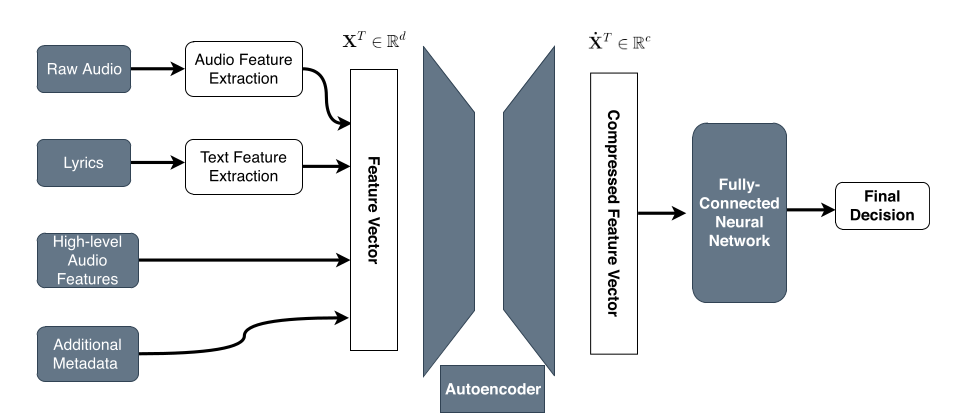
\includegraphics[width=5in]{figs/architecture.png}
%     \caption{Model architecture presented by Martin-Gutierrez et al \cite{martin-gutierrez_multimodal_2020}. We intend to replace the fully-connected CNN with an RNN.}
%     \label{architecture}
% \end{figure}


Li et al \cite{li_lstm-rpa_2021} present LSTM Rolling Prediction Algorithm (LSTM-RPA), a popularity prediction algorithm based on a Recurrent Neural Network. LSTM-RPA breaks the long-term prediction into several short-term trend predictions. This work is an important example of using an RNN architecture to predict song popularity. Wang et al \cite{wang_music_2019} also present an LSTM model for forecasting popularity.
    
Araujo et al \cite{araujo_predicting_2019} present a popularity prediction method using Support Vector Machines; this method predicts whether a song will appear on the Spotify Top 50 Global charts. This work has similar goals to our project and will serve as an important reference for evaluating our model’s accuracy.

In their 2018 paper, Choi et al \cite{choi_comparison_2018} compare audio pre-processing methods for deep neural networks. Their primary result demonstrates that many common preprocessing techniques are redundant; this conclusion will help us inform our pre-processing decisions for our project.

% 
% You need to study the current literature of your planned work. You don't have to exhaust the literature, but you need to search related work with a few proper key words.
% If there are related work, you need to cite them. For example, if you want to cite the ``Deep Learning'' book \cite{goodfellow2016deep}, then you should use the ``\textbackslash cite'' command.
% This section helps you to establish the current status of known knowledge around the project. Particularly, you may consider to cite the research work solving the same problem.  

% \section{Background} ???> Maybe??
% 
% This section is optional. If your project is related to some standard formulations, and you need to introduce details to make your later models clear, you should consider to put these \textbf{standard} formulations here.  For example, if you are going to do some modification of GRU later, but you need to have an introduction of GRU first, then it belongs to this section. A negaive example is, your project will use a GRU layer in a standard way, then a detailed introduction of GRU is not needed. 
% 
% 
% \noindent \textbf{Proposal submission:} When you submit your proposal, you should include the ``Introduction'' and ``Related Work'' sections. If you have a ``Background'' section, you should include it as well. The rubrics for grading your proposal include: 
% \begin{itemize}
% \item 2 points if you have a clear motivation
% \item 3 points if you have a clear summary of your project 
% \item 3 points if you have done at least a rough literature study 
% \item 2 points for the readability of your project (you can use Grammarly to correct your grammar issues.) 
% \end{itemize}
% 
\section{Methods}

\subsection{Dataset}
Our primary dataset is a modified version of the daily top 200 songs by stream count in the Philippines, from January 1st 2017 to May 20th 2021 \cite{peralta_spotify_nodate}. We reshaped this dataset to be of the form $\mathbb{R}^{d \times s}$, where $d$ is the number of dates in the dataset and $s$ is the number of songs.

One issue with this dataset is that it only represents the top 200 songs for a given day; as a result, songs occasionally drop off the charts for a few days and then return, leaving gaps in our time series. To solve this, we interpolated values for gaps of size exactly one (representing one day of off-chart stream counts) and filtered out songs containing zero values greater than a strict threshold. Due to the sparsity of our data, we experimented with different thresholds for including a song resulting, in a variety of different values for $s$.

% The format of the data at this point is tensor of the shape [Timesteps, Stream Count By Song]. The data was still incredibly sparse and in order to further avoid this problem and to form a training and testing set we scanned out data sets for songs which achieved a certain threshold entries over the course of the time.

To formulate our training data, we took sub-sequences of the overall date sequence for each song, with subsequences each of size \texttt{lookback} in our training dataset and the next timestep (of length one) set as the target value.

 After trimming our data set in such a manner the shape is 
\[X = [\text{Batch Size, Lookback, $s$}]\]
\[Y = [\text{Batch Size, 1, $s$}]\]
where $X$ is our training data and $Y$ is our target data.

In order to test our hypothesis, one of our architectures has multiple inputs. The second data was formed by obtaining a variety of metadata for each song in the original dataset from the Spotify API. This metadata includes features such as dancibility or acousticness in the form of a real value from 0 to 1. For each of the songs, we extracted 13 metadata features and produced a tensor of shape [$s$, 13].

\subsection{Model Architecture}

The learning problem is a straightforward regression problem. Given the daily stream counts of songs over a period of time, we are looking to accurately predict the stream count of the next day. Given the time-oriented nature of the problem, our models consist of recurrent layers. We built basic models using both LSTMs and GRUs to produce baseline accuracy metrics to be used to evaluate our multiple-input models. 

\begin{figure}
    \centering{}
    % \includegraphics{}
    \caption{TODO: LSTM and GRU summaries}
\end{figure}

We propose an architecture for a multi-input model that combines stream-count data with the extracted metadata. We first run the stream count information through a recurrent neural network. Then we concatenate the output from this model with the $m$ metadata features to create a feature vector of length $m + 1$. Then we feed this feature vector through a feed-forward neural network to output an improved stream count prediction.

\begin{figure}
    \centering{}
    % \includegraphics{}
    \caption{TODO: better-drawn version of architecture}
\end{figure}

\subsection{Model Evaluation}
We used Mean Squared Error, Root Mean Squared Error, and Mean Absolute Error as our evaluation metrics. 

Additionally, we visualize the predictions of our model by plotting the predictions alongside the original stream counts.


% 
% This section should be a detailed introduction of your project. This section should only contain your own work. For example, if you have modified a GRU architecture, this section should only have the modification of GRU. The original GRU structure should be put in the ``Background'' section.  
% 
% In this section, you should have a rigorous introduction of your problem. This list of questions help you to do the formulation,
% \begin{itemize}
% \item What data do you have? How are they denoted ($X$ represents features)? Is every notation well defined (e.g. $X \in \mathcal{R}^d$)? 
% \item What type learning problem it is? What's the desired output from the model? 
% \item What's the input to the model? Is it the same as (part of) the data? Any processing before you can feed the data to the model?
% \item What the model? If the model is not a standard one, do you have a function form of the model?
% \item What's the loss function of the model? If it is not a standard problem, you need to use an equation to show that exactly. 
% \item Can you check all symbols to make sure that every one is well defined?
% \end{itemize}
% 
% 
\section{Experiments}

\subsection{GRU and LSTM}
% TODO: add experimentation with basic LSTM and GRU 



\begin{tabular}{| c  c  c |}
    \hline
     & LSTM  & GRU \\ 
     \hline 
     RMSE & & \\ 
     MAE & & \\  
     \hline
\end{tabular}

\subsection{Multiple-Input Models}
% TODO: results for joint model 


Our first major attempt to improve performance was to train the multiple input model, which was previously described. This did not yield satisfactory results and was not properly training. % TODO: revisit this as a group 

 There are two intuition as to why the model did not work. The first being that since the recurrent layers are deeper in the model then we have no control over how they train. Therefore they may not be training to predict stream count and rather some other value. The other major issue is that since the RNN is only producing one value which is being concatenated onto the metadata for each song, than the model is going to naturally give more weight to the 13 metadata variables. 
% 
% TODO: loss 
\begin{figure}[h]
    \centering 
    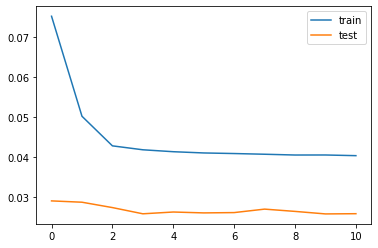
\includegraphics[width=3in]{figs/loss.png}
    \caption{Training and Testing loss (MSE)}
\end{figure}

% TODO: sample graphs 
% TODO: output metrics 
% TODO: comparison between sequential, functional, meta, no meta
% TODO: other model tweaks 


% TODO: plots here 
\begin{figure}[h]
    \centering
    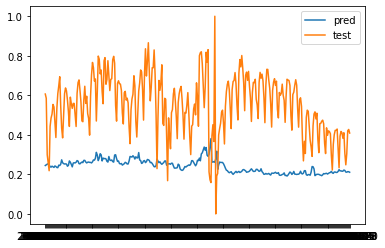
\includegraphics[width=3in ]{figs/stream_count_PLACEHOLDER}
    \caption{Predicted stream counts and validation data }
\end{figure}

% 
% In this section, you should report your experiments, which that are either related to your hypotheses or the evaluation measures of your models. Do NOT manipulate experiment results, and its OK that the experiment results do not support your hypotheses or expectations. For example, if your project is a modification of the GRU and argues that the motivation can improve its performance. However, the experiment results do not show so. In this section, you should report your observations in experiments. Then you should analyze the results in either of the following ways:
% \begin{itemize}
% \item the original argument is still correct, but experiments are not perfect. There is still a chance that the modification should work.  
% \item the original argument is invalid by observing experiment results. Some part of the argument is wrong. If there is a fix, you can also talk about further modifications.  
% \end{itemize}
% 
\section{Conclusion}
\textbf{Something about successful vs unsuccessful models}


While we were unsuccessful in our attempts to use the metadata of the song to improve performance that may mostly be due to implementation issues. As such it could certainly benefit from further attempts. One potential modification to the multi-input model is to train the recurrent layers as a separate model for a preliminary input. Then proceed to train a model which uses that output alongside the metadata to refine the predicted value. This avoids the issue of not knowing how the recurrent layer is training in the larger model, but still may present the problem that more weight is being given to the metadata than the predicted value. As well a larger and less sparse data set could be used a most likely would improve performance.
While adding more data would improve the performance it could also lead to complications due to differing music tastes across different regions. By focusing on the Philippines data set  

% TODO: which models were successful and how successful 
% TODO: reiterate the WHY 
% TODO: future work discussion 

% Draw conclusions from this project. Summarize the new findings you want your reader to learn.  
% 
\section{Share of work}
% 
% If the team has more than person, then you should report who has done which part of work. Particularly, you should mention these work items. If multiple people participated in one item, then you can list the percentage of contribution of each person. 
% 
% \begin{itemize}
% \item writing of the proposal 
% \item coding
% \item running experiments and collecting data 
% \item discussions (of project ideas and experiment results) 
% \item writing of the final report 
% \end{itemize}

\bibliographystyle{plain}
\bibliography{sample}

\end{document}
